\FloatBarrier\section{Mapeamento da Solução e Arquitetura}
O navegador carrega um painel que consulta periodicamente a rota de identificação da API. O endereço usado pelo cliente permanece estável quando um pod é substituído. Isso é possível porque o Service da aplicação recebe conexões pela porta publicada no nó e encaminha o tráfego para pods selecionados por rótulo. O processo HTTP recebe a conexão na porta interna do contêiner. A Figura~\ref{fig:arquitetura} acompanha a consulta que resulta em escrita.
\begin{figure}[!ht]\centering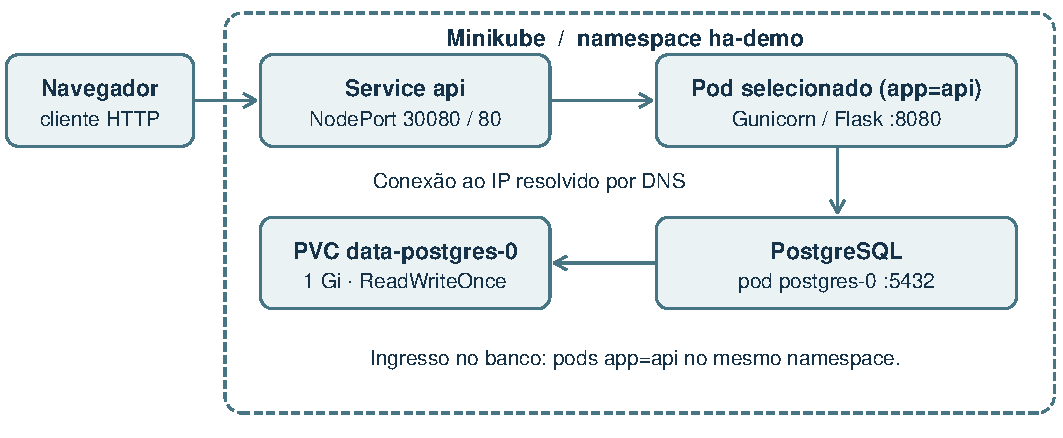
\includegraphics[width=\linewidth]{figuras/arquitetura-final.pdf}
\caption{Percurso de uma visita a partir dos objetos declarados no projeto. A seta entre API e banco representa a conexão aberta após a descoberta do endereço pelo Service interno. A seta para o PVC representa a montagem do armazenamento.}\label{fig:arquitetura}\end{figure}

Cada réplica obtém do Kubernetes sua identidade, seu IP e o nome do nó. Ao receber a consulta, a aplicação abre uma conexão ao PostgreSQL por nome de serviço, insere uma linha com a identificação do pod e lê a quantidade de linhas. A resposta combina dados locais, como a identidade de quem atendeu, com um dado compartilhado, a contagem. Fechar a conexão HTTP após a resposta dá à próxima conexão outra oportunidade de seleção de destino. A escolha pode voltar ao mesmo pod. Por isso, a alternância de identidades é uma observação mais informativa que a expectativa de uma ordem circular fixa.

O Service do banco é interno e do tipo \textit{headless}: oferece descoberta por DNS para alcançar o pod do PostgreSQL. A política de ingresso permite a porta do banco aos pods com o rótulo da aplicação no mesmo namespace. Há duas verificações em camadas diferentes: alcançar a porta permite iniciar a comunicação, enquanto executar a escrita exige uma sessão válida no banco. O PostgreSQL mantém seus arquivos num volume reservado ao primeiro membro do StatefulSet. Um pod recriado com a mesma identidade ordinal pode remontar esse volume e abrir o conjunto de dados existente.

A Figura~\ref{fig:objetos} detalha a distribuição das responsabilidades. Cada pod da API contém o processo de atendimento e um contêiner de inicialização que termina antes dele. Os parâmetros comuns chegam pelo ConfigMap e pelo Secret. O Service seleciona as réplicas disponíveis; o Deployment governa sua quantidade. Na camada persistente, o StatefulSet postgres gerencia o pod postgres-0 e associa sua identidade ordinal ao claim data-postgres-0 (ambos representados na faixa inferior do diagrama). As setas de configuração e controle não representam tráfego de visitas.

\begin{figure}[!ht]\centering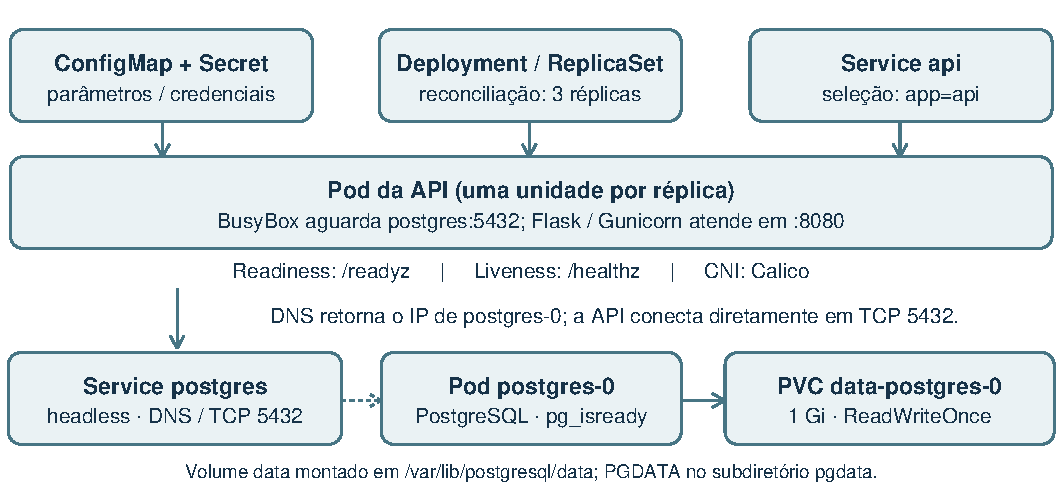
\includegraphics[width=\linewidth]{figuras/objetos-final.pdf}\caption{Arquitetura dos componentes Kubernetes utilizados no projeto. As setas superiores indicam, respectivamente, injeção de configuração, controle de réplicas e encaminhamento HTTP. O trecho pontilhado inferior identifica o pod postgres-0 (gerenciado pelo StatefulSet postgres e vinculado ao PVC data-postgres-0) descoberto pelo Service headless. A API verifica prontidão em /readyz e vivacidade em /healthz.}\label{fig:objetos}\end{figure}

O momento da falha também importa. Antes de iniciar a API, um contêiner de inicialização espera que a porta do banco aceite conexão. Após a inicialização, a sonda de prontidão da API verifica o servidor web independentemente do banco. Se uma gravação falhar, a aplicação ainda consegue devolver a identidade do pod e indicar que a contagem está indisponível. Portanto, uma queda do banco pode permitir atendimento parcial pelas réplicas existentes e simultaneamente retardar a entrada de novas réplicas. A segunda consequência decorre da configuração de inicialização; o comportamento registrado durante a queda é discutido na Seção~\ref{sec:dados}.

A arquitetura dispõe de várias réplicas HTTP, mas concentra as escritas em uma instância do PostgreSQL. Recriar essa instância sobre o volume existente exige um intervalo de inicialização. Também há dependência do nó que executa o laboratório. São duas fronteiras de falha diferentes daquela exercitada ao remover apenas uma réplica HTTP.
